
\documentclass[a4paper,12pt]{article}
\usepackage{pgfplots}
\usepackage{graphicx}
\pgfplotsset{compat=1.18}
\usepackage[utf8]{inputenc}
\usepackage{amsmath, subcaption, amssymb, graphicx, booktabs, pgfplots, pgfplotstable, float}
\usepackage{geometry}
\geometry{left=2cm, right=2cm, top=2.5cm, bottom=2.5cm}
\renewcommand{\figurename}{Figura}
\renewcommand{\tablename}{Tabla}

\title{Relación de Problemas 2. Estadística descriptiva bidimensional. Regresión y correlación}
\author{Salvador Gil Antonio \and Salvador Gil Sergio \and Serantes Rivas Víctor\\\\Estadística Descriptiva e Introducción a la Probabilidad \\ Primer curso del Doble Grado en Ingeniería Informática y Matemáticas}

\begin{document}

\maketitle
\section*{Ejercicio 1}
Se han lanzado dos dados varias veces, obteniendo los siguientes resultados:

\noindent
\textbf{X:} 1 2 2 3 5 4 1 3 3 4 1 2 5 4 3 4 4 5 3 1 6 5 4 6 \\
\textbf{Y:} 2 3 1 4 3 2 6 4 1 6 6 5 1 2 5 1 1 2 6 6 2 1 2 5

\begin{enumerate}
    \item[a)] Construir la tabla de frecuencias.
    \item[b)] Calcular las puntuaciones medias obtenidas con cada dado y ver cuáles son más homogéneas.
    \item[c)] ¿Qué resultado del segundo dado es más frecuente cuando en el primero se obtiene un 3?
    \item[d)] Calcular la puntuación máxima del 50\% de las puntuaciones más bajas obtenidas con el primer dado si con el segundo se ha obtenido un 2 o un 5.
\end{enumerate}

Este ejercicio con el enunciado original no tiene ningún sentido, ya que es absurdo asumir una relación entre los resultados de dos dados distintos. Para proceder, cambiamos el enunciado, teniendo ahora como variable X el número de horas estudiadas diarias de un estudiante de primero del Doble Grado en Ingeniería Informática y Matemáticas el primer cuatrimestre, y la variable Y el número de asignaturas aprobadas ese cuatrimestre.

\begin{enumerate}
    \item[a)] Construir la tabla de frecuencias.
\end{enumerate}

\begin{center}
\begin{tabular}{c|cccccc|c||c|c}
\textbf{X\textbackslash Y} & 1 & 2 & 3 & 4 & 5 & 6 & $n_{i.}$ & $x_in_{i.}$& $n_i(x_i- \bar x)^2$\\
\hline
1 & 0 & 1 & 0 & 0 & 0 & 3  & 4 & 4&22,5625\\
2 & 1 & 0 & 1 & 0 & 1 & 0  & 3 & 6 &5,6718\\
3 & 1 & 0 & 0 & 2 & 1 & 1  & 5 & 15 & 0,7031\\
4 & 2 & 3 & 0 & 0 & 0 & 1  & 6 & 24 & 2,3437\\
5 & 2 & 1 & 1 & 0 & 0 & 0  & 4 & 20 & 10,5625\\
6 & 0 & 1 & 0 & 0 & 1 & 0  & 2 & 12 & 13,78125\\
\hline
$n_{.j}$ & 6 & 6 & 2 & 2 & 3 & 5 & 24 & 81 &55,52485\\
\hline
$y_jn_{.j}$ & 6 & 12 & 6 & 8 & 15 & 30 & 17&\\
\hline
$n_i(x_i- \bar x)^2$ & 29,2515&8,7555 &0,0685&1,254&9,6337&38,976&87,9567&\\
\end{tabular}
\end{center}

\begin{enumerate}
    \item[b)] Calcular las puntuaciones medias obtenidas con cada dado y ver cuáles son más homogéneas.
\end{enumerate}

Una vez calculadas las distribuciones marginales, fácilmente obtenemos las medias $\bar x=3,375$, $\bar y = 3,208$.\\
Para ver cuál de las dos es más homogénea, utilizamos las medias para calcular el Coeficiente de Variación de Pearson de cada una de las distribuciones marginales. Para ello, primero calculamos las varianzas:
$\sigma_x^2=\frac{55,52485}{24}=2,313535$, $\sigma_y^2=\frac{87,9567}{24}=3,66486$.\\
Finalmente, vemos qué Coeficiente de Variación de Pearson es menor: $C.V_x=\frac{\sigma_x}{|\bar x|}= 0,45067 < C.V_y=\frac{\sigma_y}{|\bar y|}=0,59675$, por lo que la distribución marginal de la variable X es más homogénea.\\

\begin{enumerate}
    \item[c)] ¿Qué resultado del segundo dado es más frecuente cuando en el primero se obtiene un 3?
\end{enumerate}

Tenemos que calcular la moda de la distribución condicionada a que x=3, que es $Mo_{x=3}=4$\\


\begin{enumerate}
    \item[d)] Calcular la puntuación máxima del 50\% de las puntuaciones más bajas obtenidas con el primer dado si con el segundo se ha obtenido un 2 o un 5.
\end{enumerate}

Tenemos que calcular la mediana de la distribución de Y condicionada a que y = 2 o que y = 5:

\begin{center}
\begin{tabular}{c|c|c}
$x_i$ & $n_{i2}+n_{15}$&$N_i$ \\
\hline
1 & 1 & 1 \\
2 & 1 & 2 \\
3 & 1 & 3 \\
4 & 3 & 6 \\
5 & 1 & 7 \\
6 & 2 & 9 \\
\hline
&9&\\
\end{tabular}
\end{center}

Y como no hay ningún valor que cumpla que $N_i = \frac{N}{2} = 4,5$, el valor de la mediana será el inmediatamente superior, es decir $Me_{x =2, x=5}=4$ 

\section*{Ejercicio 2}
Medidos los pesos ($X$, en kg) y las alturas ($Y$, en cm) de un grupo de individuos, se obtiene:

\begin{center}
\begin{tabular}{c|cccccc|ccc}
X $\backslash$ Y & 160 & 162 & 164 & 166 & 168 & 170 & $n_i.$ & $x_in_i$ & $n_i(x_i- \bar y)$ \\
\hline
48 & 3 & 2 & 2 & 1 & 0 & 0 & 8 & 384 & 304.68 \\
51 & 2 & 3 & 4 & 2 & 2 & 1 & 14 & 714 & 140.808\\
54 & 1 & 3 & 6 & 8 & 5 & 1 & 24 & 1296 & 0.7050\\
57 & 0 & 0 & 1 & 2 & 8 & 3 & 14 & 798 & 112.01\\
60 & 0 & 0 & 0 & 2 & 4 & 4 & 10 & 600 & 847.928\\
\hline
$n.j$ & 6 & 8 & 13 & 15 & 19 & 9 & 70 & 3792 & 847.928\\
$y_nn._j$ & 960 & 1296 & 2132 & 2490 & 3192 & 1530 & 11600\\
$n._j(y_j-\bar y)$ & 195.89 & 110.55 & 38.141 & 1.226 & 49.29 & 165.32 & 610.26\\
\end{tabular}
\end{center}

\begin{enumerate}
    \item[a)] Calcular el peso medio y la altura media y decir cuál es más representativo.\\
    Peso medio:
    $$\bar x = \frac {1}{n} \sum\limits_{i = 1}^k {x_i n_i} = 54.1714kg$$
    Altura media:
    $$\bar y = \frac {1}{n} \sum\limits_{j = 1}^k {y_j n_j} = 165.714cm$$

    Para ver cuál es más representativo, calculamos el C.V de Pearson con respecto a la media aritmética:
    $$\sigma_x^2 = {\frac{1}{n}\sum\limits_{i=1}^kn_i(x_i-\bar x)^2} = 12.827kg^2$$
    $$CV_x = \frac {\sigma_x}{|\bar x|} = 0,066113$$

    $$\sigma_y^2 = {\frac{1}{n}\sum\limits_{j=1}^kn_i(y_j-\bar y)^2} = 8.7181cm^2$$
    $$CV_y = \frac {\sigma_y}{|\bar y|} = 0,01781$$

    Como el Coeficiente de Variación de Pearson de la altura es menor, quiere decir que la media aritmética de la variable Y es más representativa de la distribución que la de la variable X.
    
    \item[b)] Calcular el porcentaje de individuos que pesan menos de 55 kg y miden más de 165 cm.\\
    Como los valores inmediatamente inferiores a 55kg (54kg) y superiores a 165cm (166cm) aparecen en la tabla, simplemente tendremos que calcular el porcentaje de individuos que se cumplen las condiciones deseadas.
    Lo calculamos usando la tabla de la distribución condicionada a que $i$ $<$ 4 y $j$ $>$ 3:

    \begin{center}
    \begin{tabular}{c|cccccc|ccc}
    X $\backslash$ Y &166 & 168 & 170 & $n_i.$\\
    \hline
    48 & 1 & 0 & 0 & 1\\
    51 & 2 & 2 & 1 & 5\\
    54 & 8 & 5 & 1 & 14\\
    \hline
    $n._j$ & 11 & 7 & 2 & 20
    \end{tabular}
    \end{center}

    El porcentaje será:
    $$100 \frac{20}{70} = 28.57\%$$
    
    \item[c)] Entre los que miden más de 165 cm, ¿cuál es el porcentaje de los que pesan más de 52 kg?\\

    Comenzamos haciendo la tabla de la distribución condicionada a que $Y > 165$:

    \begin{center}
    \begin{tabular}{c|cccccc|ccc}
    X $\backslash$ Y &166 & 168 & 170 & $n_i.$\\
    \hline
    48 & 1 & 0 & 0 & 1\\
    51 & 2 & 2 & 1 & 5\\
    54 & 8 & 5 & 1 & 14\\
    57 & 2 & 8 & 3 & 13\\
    60 & 2 & 4 & 4 & 10\\
    \hline
    $n._j$ & 15 & 19 & 9 & 43\\
    \end{tabular}
    \end{center}

    Ahora calculamos el percentil en el que se encuentran los individuos cuyo peso es menor o igual a $52kg$:

    $$52 = 51 + \frac{\frac{x}{100}- 6}{14}(3) \Rightarrow x = 10.667\% $$

    Por tanto, el porcentaje de individuos cuyo peso es mayor a $52kg$ es:
    $$100 - 10.667=89.33\%$$
    
    \item[d)] ¿Cuál es la altura más frecuente entre los individuos cuyo peso oscila entre 51 y 57 kg?\\
    Calculamos la moda de la distribución condicionada a que 1$<i<$5.

    \begin{center}
    \begin{tabular}{c|cccccc|ccc}
    X $\backslash$ Y & 160 & 162 & 164 & 166 & 168 & 170 & $n_i.$\\
    \hline
    51 & 2 & 3 & 4 & 2 & 2 & 1 & 14\\
    54 & 1 & 3 & 6 & 8 & 5 & 1 & 24\\
    57 & 0 & 0 & 1 & 2 & 8 & 3 & 14\\
    \hline
    $n.j$ & 3 & 6 & 11 & 12 & 15 & 5 & 52 \\
    \end{tabular}
    \end{center}

    La moda es $max$ {$n._j$}$=168$
    
    \item[e)] ¿Qué peso medio es más representativo, el de los individuos que miden 164 cm o el de los que miden 168 cm?\\

    Calculamos el C.V de Pierson respecto de la media aritmética de las distribuciones condicionadas a que el peso es 164cm y 168cm respectivamente:\\
    
    $$Y=164:$$
\begin{center}
    \begin{tabular}{cccc}
    $x_i$ & $n_i$ & $x_in_i$ & $n_i(x_i-\bar x)$ \\
    \hline
    48 & 2 & 96 & 38.43\\ 
    51 & 4 & 204 & 7.661\\
    54 & 6 & 324 & 15.668\\
    57 & 1 & 57 & 21.307\\
    60 & 0 & - & -\\
    \hline
     & 15 & 681 & 83.066\\
    \end{tabular}
    \end{center}
    
    $\bar x = 52.384$, $\sigma_x^2=6.389$
    $$CV_X= \frac{\sigma_x^2}{|\bar x|} = 0.121$$
    
    $$Y=168:$$
\begin{center}
    \begin{tabular}{cccc}
    $x_i$ & $n_i$ & $x_in_i$ & $n_i(x_i-\bar x)$ \\
    \hline
    48 & 0 & - & -\\ 
    51 & 2 & 102 & 54.288\\
    54 & 5 & 270 & 24.42\\
    57 & 8 & 436 & 4.9928\\
    60 & 4 & 240 & 57.4564\\
    \hline
     & 19 & 1068 & 141.1572\\
    \end{tabular}
    \end{center}
    $\bar x = 56.21$, $\sigma_x^2=7.429$
    $$CV_X= \frac{\sigma_x^2}{|\bar x|} = 0.1321$$

    Por tanto, como el Coeficiente de variación de la distribución condicionada a que $Y=164$ es menor, su media aritmética será más representativa.
    
\end{enumerate}

\section*{Ejercicio 3}
\begin{center}
\begin{tabular}{c|cccc}
X $\backslash$ Y & 1 & 2 & 3 & 4 \\
\hline
1 & 7 & 0 & 0 & 0 \\
2 & 10 & 2 & 0 & 0 \\
3 & 11 & 5 & 1 & 0 \\
4 & 10 & 6 & 6 & 0 \\
5 & 8 & 6 & 4 & 2 \\
6 & 1 & 2 & 3 & 1 \\
7 & 1 & 0 & 0 & 1 \\
8 & 0 & 0 & 1 & 1 \\
\end{tabular}
\end{center}

\begin{enumerate}
    \item[a)] Calcular la recta de regresi\'on de $Y$ sobre $X$.
    \item[b)] \textquestiondown Es adecuado suponer una relaci\'on lineal para explicar el comportamiento de $Y$ a partir de $X$?
\end{enumerate}

\begin{center}
\begin{tabular}{c|cccc|c||c|c|c|c}

X $\backslash$ Y & 1 & 2 & 3 & 4 & $n_{i.}$ & $x_in_{i.}$ & $n_{i.}(x_i-\bar x)^2$ & $\sum n_{ij} y_{j.}$ & $x_i\sum n_{ij} y_{j.}$ \\
\hline
1 & 7 & 0 & 0 & 0 &7&7&56,566&7&7\\
2 & 10 & 2 & 0 & 0 &12&24&40,7465&14&28\\
3 & 11 & 5 & 1 & 0 & 17&51&12,0724&24&72\\
4 & 10 & 6 & 6 & 0 &22&88&0,54435&40&160\\
5 & 8 & 6 & 4 & 2 &20&100&26,786&40&200\\
6 & 1 & 2 & 3 & 1 &7&42&32,577&18&108\\
7 & 1 & 0 & 0 & 1 &2&14&19,9370&5&35\\
8 & 0 & 0 & 1 & 1 &2&16&34,566&7&56\\
\hline 
$y_{.j}$ & 48 & 21 & 15 &5&89&324&223,795&155&666\\
\hline
$n_{.j}y_j$ & 48 & 42 &45&20 & 155\\
\hline
$n_{.j}(y_j - \bar y)^2$ & 26,391 & 1,403 & 23,757 & 25,504 &77,055\\
\end{tabular}

\end{center}

\begin{enumerate}
    \item[a)] Calcular la recta de regresi\'on de $Y$ sobre $X$.
\end{enumerate}

Una vez calculadas las distribuciones marginales de X e Y, con los datos obtenidos en la tabla, calculamos las medias: $\bar x = \frac{342}{89}=3,8427$, $\bar y = \frac{155}{89}=1,7415$.\\
Ya obtenidas las medias, calculamos las varianzas (la varianza de Y todavía no hace falta, pero la calcularemos, ya que es necesaria para el apartado siguiente): $\sigma_x^2 = 2,514$, $\sigma_y^2 = 0,8657$.\\
Ahora, calculamos la covarianza: $\sigma_{xy}=m_{11}-\bar x \bar y = \frac{1}{89} x_i\sum n_{ij} y_{j.} - \bar x \bar y = 0,791084$\\
Con eso, podemos calcular la recta de regresión de Y sobre X:
\[y=\frac{\sigma_{xy}}{\sigma_x^2}+(\bar y - \frac{\sigma_{xy}}{\sigma_x^2} \bar x) = 0,3146x + 0,5323\]

\begin{enumerate}
    \item[b)] \textquestiondown Es adecuado suponer una relaci\'on lineal para explicar el comportamiento de $Y$ a partir de $X$?
\end{enumerate}

Para ver si es adecuado suponer una relación lineal para explicar el comportambiento de Y a partir de X debemos calcular el coeficiente de correlación lineal $r= \frac{\sigma_{xy}}{\sigma_x \sigma_y}=0,529150$, que no se acerca mucho a 1 por lo que no existe una relación lineal entre las dos variables.

\section*{Ejercicio 4}
Se realiza un estudio sobre la tensi´on de vapor de agua (Y , en ml. de Hg.) a distintas temperaturas
(X, en ºC). Efectuadas 21 medidas, los resultados son:
\begin{center}
\begin{tabular}{c|ccc}
X $\backslash$ Y & (0.5, 1.5] & (1.5, 2.5] & (2.5, 5.5] \\
\hline
(1, 15] & 4 & 2 & 0 \\
(15, 25] & 1 & 4 & 2 \\
(25, 30] & 0 & 3 & 5 \\
\end{tabular}
\end{center}

Explicar el comportamiento de la tensi\'on de vapor en t\'erminos de la temperatura mediante una funci\'on lineal. \textquestiondown Es adecuado asumir este tipo de relaci\'on?\\

Antes de comenzar a resolver el ejercicio, vamos a suponer que los datos de la variable Y han sido dados en mmHg, la magnitud correcta de medida\\


\begin{center}
\resizebox{.9\textwidth}{!}{
\begin{tabular}{c|ccc|c||c|c|c|c|c}
X $\backslash$ Y &(0.5, 1.5]&(1.5, 2.5]&(2.5, 5.5]& $n_{i.}$ & $x_i$ & $x_in_{i.}$ & $n_{i.}(x_i-\bar x)^2$ & $\sum n_{ij} y_{j.}$ & $x_i\sum n_{ij} y_{j.}$ \\
\hline
(1, 15] & 4 & 2 & 0 & 6 & 8 & 48 & 783,673 & 8 & 64 \\
(15, 25] & 1 & 4 & 2 & 7 & 20 & 140 & 2,28572 & 17 & 340 \\
(25, 30] & 0 & 3 & 5 & 8 & 27,5 & 220 & 521,1838 & 26 & 715\\
\hline 
$n_{.j}$ & 5 & 9  & 7 &21 &  & 408 & 1307,1425 & &1119 \\
\hline
$y_{j}$&1&2&4&&\\
\hline
$n_{.j}y_j$ & 5 & 18 & 28 &51 & \\
\hline
$n_{.j}(y_j - \bar y)^2$ & 10,204 & 1,653 & 17,2857 & 29,153 &\\
\end{tabular}
}
\end{center}

El enunciado nos pide calcular la recta de regresión de Y sobre X. Para ello, realizamos la tabla completa, de la que podemos sacar las medias: $\bar x = \frac {408}{21}= 19,42857$, $\bar y = \frac{51}{21}=2,42857$.\\
Ahora con las medias, calculamos las varianzas: $\sigma_x^2=\frac{1307,1425}{21}=62,4$, y $\sigma_y^2=\frac{29,142}{21}=1,17801$.\\
Por último, calculamos la covarianza: $\sigma_{xy}=\frac{1}{21} x_i\sum n_{ij}y_j - \bar x \bar y = \frac{1119}{21} - 19,42857*2,42857 = 6,1088$.\\
Finalmente, ahora que tenemos todo lo necesario, podemos calcular la recta de regresión de Y sobre X: $y=\frac{\sigma_{xy}}{\sigma_x^2}+(\bar y - \frac{\sigma_{xy}}{\sigma_x^2} \bar x) = 0,098x+0,51$\\

Para ver si es adecuado asumir ese tipo de relación, calculamos el coeficiente de correlación lineal $r^2=(\frac{\sigma_{xy}}{\sigma_x \sigma_y})^2 = 0,431$. Como $r^2$ no se acerca a 1, este tipo de ajuste no es muy adecuado.

\section*{Ejercicio 5}
Estudiar la dependencia o independencia de las variables en cada una de las siguientes distribuciones. Dar, en cada caso, las curvas de regresi\'on y la covarianza de las dos variables.

\textbf{Distribuci\'on 1}
\begin{center}
\begin{tabular}{c|ccccc}
X $\backslash$ Y & 1 & 2 & 3 & 4 & 5 \\
\hline
10 & 2 & 4 & 6 & 10 & 8 \\
20 & 1 & 2 & 3 & 5 & 4 \\
30 & 3 & 6 & 9 & 15 & 12 \\
40 & 4 & 8 & 12 & 20 & 16 \\
\end{tabular}
\end{center}

\textbf{Distribuci\'on 2}
\begin{center}
\begin{tabular}{c|ccc}
X $\backslash$ Y & 1 & 2 & 3 \\
\hline
$-1$ & 0 & 1 & 0 \\
0 & 1 & 0 & 1 \\
1 & 0 & 1 & 0 \\
\end{tabular}
\end{center}

Antes de nada, en la primera distribución nos damos cuenta de que $f_{ij}=f_{i.}f_{.j}=\frac{n_{i.}n_{.j}}{n}$, lo que significa que las dos variables son independientes, y no tendría ningún sentido trabajar con ellas.\\

\begin{center}
\begin{tabular}{c|ccc|c||c|c|c}
X $\backslash$ Y & 1 & 2 & 3 & $n_{i.}$ & $x_in_{i.}$ & $\sum n_{ij} y_{j.}$ & $x_i\sum n_{ij} y_{j.}$ \\
\hline
-1 & 0 & 1 & 0 & 1 & -1 & 2 & -2 \\
0 & 1 & 0 & 1 & 2 & 0 & 4 & 0\\
1 & 0 & 1 & 0 & 1 & 1 & 2 & 2\\
\hline
$n{.j}$ & 1 & 2 &  1 & 4 & 0 & & 0\\
\hline
$y_jn_{.j}$ & 1 & 4 & 3 & 8 & &\\
\end{tabular}
\end{center}

La curva de regresión de Y sobre X son los puntos $(\bar x_i, y_j)$, que son:
\[\{(-1,2), (0,2), (1,2)\}\]


\begin{center}
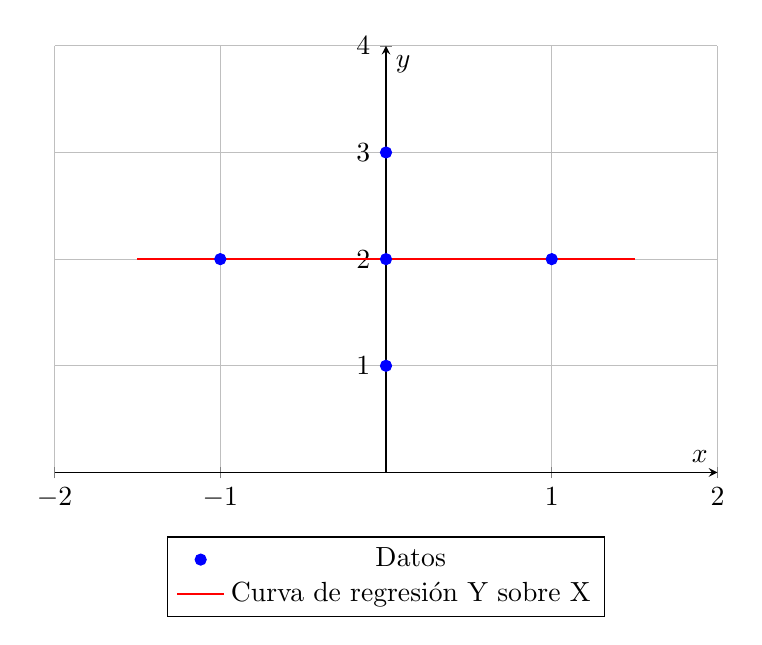
\begin{tikzpicture}
  \begin{axis}[
    axis lines = middle,
    xlabel = $x$,
    ylabel = $y$,
    xmin = -2, xmax = 2,
    ymin = 0, ymax = 4,
    grid = both,
    width=10cm,
    height=7cm,
    legend style={at={(0.5,-0.15)},anchor=north},
    xtick={-2,-1,0,1,2},
    ytick={0,1,2,3,4}
  ]
    % Puntos
    \addplot[only marks, mark=*, blue] coordinates {(-1,2) (0,2) (1,2) (0,3) (0,1)};
    \addlegendentry{Datos}

    % Curva de regresión (recta horizontal)
    \addplot[red, thick, domain=-1.5:1.5] {2};
    \addlegendentry{Curva de regresión Y sobre X}
  \end{axis}
\end{tikzpicture}\\
\end{center}


La curva de regresión de X sobre Y son los puntos $(x_i,\bar  y_j)$, que son:
\[\{(0,1), (0,2), (0,3)\}\]

\begin{center}
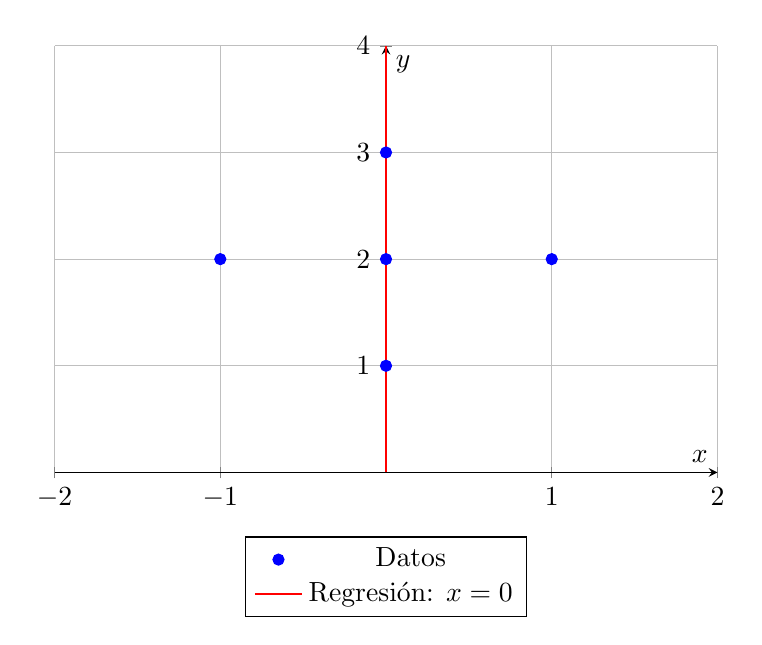
\begin{tikzpicture}
  \begin{axis}[
    axis lines = middle,
    xlabel = $x$,
    ylabel = $y$,
    xmin = -2, xmax = 2,
    ymin = 0, ymax = 4,
    grid = both,
    width=10cm,
    height=7cm,
    legend style={at={(0.5,-0.15)},anchor=north},
    xtick={-2,-1,0,1,2},
    ytick={0,1,2,3,4}
  ]
    % Puntos
    \addplot[only marks, mark=*, blue] coordinates {(-1,2) (0,2) (1,2) (0,3) (0,1)};
    \addlegendentry{Datos}

    % Curva de regresión (recta horizontal)
    \addplot[red, thick] coordinates {(0,0) (0,4)};
    \addlegendentry{Regresión: $x = 0$}
  \end{axis}
\end{tikzpicture}\\
\end{center}

La covarianza de la segunda distribución es $\sigma_{xy}=\frac{1}{n} x_i\sum n_{ij}y_j - \bar x \bar y = \frac{1}{n}*0 - 0 = 0$\\

\section*{Ejercicio 6}
\begin{center}
\begin{tabular}{c|cccc}
X $\backslash$ Y & 1 & 2 & 3 & 4 \\
\hline
10 & 1 & 3 & 0 & 0 \\
12 & 0 & 1 & 4 & 3 \\
14 & 2 & 0 & 0 & 2 \\
16 & 4 & 0 & 0 & 0 \\
\end{tabular}
\end{center}

\begin{enumerate}
    \item[a)] \textquestiondown Son estad\'isticamente independientes $X$ e $Y$?
    \item[b)] Calcular y representar las curvas de regresi\'on de $X/Y$ e $Y/X$.
    \item[c)] Cuantificar el grado en que cada variable es explicada por la otra mediante la correspondiente curva de regresi\'on.
    \item[d)] \textquestiondown Est\'an $X$ e $Y$ correladas linealmente? Dar las expresiones de las rectas de regresi\'on.
\end{enumerate}

\begin{enumerate}
    \item[a)] \textquestiondown Son estad\'isticamente independientes $X$ e $Y$?
\end{enumerate}
Las variables, en este caso, no son estadísticamente independientes, ya que se tendría que cumplir que $f_{ij}=f_{i.}f_{.j}=\frac{n_{i.}n_{.j}}{n}$, pero en la tabla hay ceros, por lo que $\frac{n_{i.}n_{.j}}{n}=0$, mientras que $f_{ij}$ es no nulo, así que la independencia es imposible.

\begin{enumerate}
    \item[b)] Calcular y representar las curvas de regresi\'on de $X/Y$ e $Y/X$.
\end{enumerate}

La curva de regresión de Y sobre X son los puntos $(\bar x_i, y_j)$, que son:
\[\{(1,14.57), (2,10.5), (3,12), (4, 12.8)\}\]

\begin{center}
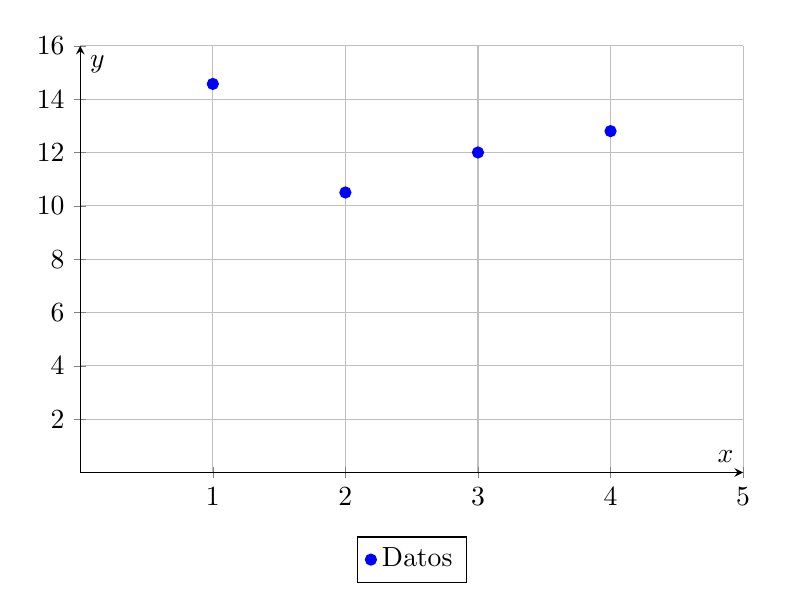
\begin{tikzpicture}
  \begin{axis}[
    axis lines = middle,
    xlabel = $x$,
    ylabel = $y$,
    xmin = 0, xmax = 5,
    ymin = 0, ymax = 16,
    grid = both,
    width=10cm,
    height=7cm,
    legend style={at={(0.5,-0.15)},anchor=north},
    xtick={0,...,5},
    ytick={0,2,...,16}
  ]
    % Puntos
    \addplot[only marks, mark=*, blue] coordinates {
      (1,14.57) (2,10.5) (3,12) (4,12.8)
    };
    \addlegendentry{Datos}
  \end{axis}
\end{tikzpicture}
\end{center}

La curva de regresión de Y sobre X son los puntos $(\bar x_i, y_j)$, que son:
\[\{(10, 1.75), (12, 3.25), (14, 2.5),(16, 1)\}\]

\begin{center}
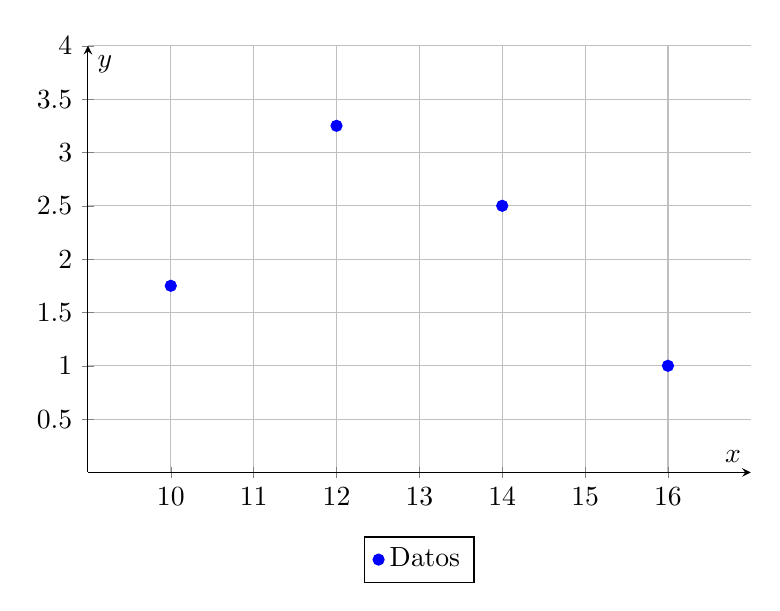
\begin{tikzpicture}
  \begin{axis}[
    axis lines = middle,
    xlabel = $x$,
    ylabel = $y$,
    xmin = 9, xmax = 17,
    ymin = 0, ymax = 4,
    grid = both,
    width=10cm,
    height=7cm,
    legend style={at={(0.5,-0.15)},anchor=north},
    xtick={10,11,...,16},
    ytick={0,0.5,...,4}
  ]
    % Puntos
    \addplot[only marks, mark=*, blue] coordinates {
      (10,1.75) (12,3.25) (14,2.5) (16,1)
    };
    \addlegendentry{Datos}
  \end{axis}
\end{tikzpicture}
\end{center}

\begin{enumerate}
    \item[c)] Cuantificar el grado en que cada variable es explicada por la otra mediante la correspondiente curva de regresi\'on.
\end{enumerate}

Primero calculamos la tabla completa con todo lo que necesitamos:

\begin{center}
\resizebox{.9\textwidth}{!}{
\begin{tabular}{c|cccc|c||c|c|c|c|c}
X $\backslash$ Y & 1 & 2 & 3 & 4 & $n_{i.}$ & $x_in_{i.}$ & $n_{i.}(x_i-\bar x)^2$ & $\sum\limits_jn_{i.}(y_j^*-\bar y_j)^2$ & $\sum n_{ij} y_{j.}$ & $x_i\sum n_{ij} y_{j.}$ \\
\hline
10 & 1 & 3 & 0 & 0 & 4 & 40 & 31,36 & 1,44 & 7 & 70\\
12 & 0 & 1 & 4 & 3 & 8 & 96 & 5,12 & 6,48 & 26 & 312\\
14 & 2 & 0 & 0 & 2 & 4 & 56 & 5,76 & 0,09 & 10 & 140\\
16 & 4 & 0 & 0 & 0 & 64 & 40,96 & 7,29 & 4 & 64\\
\hline
$n_{.j}$ & 7 & 4 & 4 & 5 & 20 & 256 & 83,2 & 15,3 & & 586\\
\hline
$n_{.j}y_j$ & 7 & 8 & 12 & 20 & 47 & & & &\\
\hline
$n_{.j}(y_l-\bar y)^2$ & 12,7575 & 0,49 & 1,69 & 13,6175 & 28,55 & & & &\\
\hline
$\sum n_{.j}(x^*-\bar x)^2$ & 21,9303 & 21,16 & 2,56 & 0 & 43,6504 & & & &\\
\end{tabular}
}
\end{center}

Tenemos que obtener $\eta^2_{X/Y}$ y $\eta^2_{Y/X}$:\\
$\sigma_{exp_y}^2 = \sum\limits_i \sum\limits_j f_{ij}(y_i^*- \bar y)^2 = \frac{1}{n} \sum\limits_i \sum\limits_j n_{ij}(y_i^*- \bar y)^2 = 0,756$, por lo que $\eta_{X/Y}^2 = \frac{\sigma_{exp_y}^2}{\sigma_y^2} = 0,53590$\\
$\sigma_{exp_x}^2 = \sum\limits_i \sum\limits_j f_{ij}(x_i^*- \bar x)^2 = \frac{1}{n} \sum\limits_i \sum\limits_j n_{ij}(x_i^*- \bar x)^2 = 2,282545$, por lo que $\eta_{Y/X}^2 = \frac{\sigma_{exp_x}^2}{\sigma_x^2} = 0,54434$\\

Como vemos, el coeficiente de determinación de Y/X es mayor, por lo que la variable Y explica mejor a la variable X\\

\begin{enumerate}
    \item[d)] \textquestiondown Est\'an $X$ e $Y$ correladas linealmente? Dar las expresiones de las rectas de regresi\'on.
\end{enumerate}

Para calcular las rectas de regresión, hacemos uso de los datos calculados en la tabla:\\
$\bar x = 12,8$, $\bar y = 2,35$. Con las medias, calculamos $\sigma_x^2 = 4,16$ y $\sigma_y^2= 1,4275$.
Finalmente calculamos la covarianza: $\sigma_{xy}= m_{11} - \bar x \bar y = -0,78$.\\
\[y = \frac{\sigma_{xy}}{\sigma_x^2}x+(\bar y -\frac{\sigma_{xy}}{\sigma_x^2})\bar x = 0,1875x+4,75)\]
\[x = \frac{\sigma_{xy}}{\sigma_y^2}y+(\bar x -\frac{\sigma_{xy}}{\sigma_y^2})\bar y = 0,5464y+14,084)\]

Ahora que tenemos las rectas de regresión, calculamos el coeficiente de correlación para ver si están correladas linealmente:\\
$r^2=(\frac{\sigma_{xy}}{\sigma_x\sigma_y})^2=0,102452677$, así que $r=-\sqrt{0,32}$. Vemos que $-1<<r<<1$, así que las variables no están correladas linealmente.\\

\section*{Ejercicio 7}
Para cada una de las siguientes distribuciones:

\textbf{Distribución A}
\begin{center}
\begin{tabular}{c|ccc}
X $\backslash$ Y & 10 & 15 & 20 \\
\hline
1 & 0 & 2 & 0 \\
2 & 1 & 0 & 0 \\
3 & 0 & 0 & 3 \\
4 & 0 & 1 & 0 \\
\end{tabular}
\end{center}

\textbf{Distribución B}
\begin{center}
\begin{tabular}{c|ccc}
X $\backslash$ Y & 10 & 15 & 20 \\
\hline
1 & 0 & 2 & 0 \\
2 & 1 & 0 & 0 \\
3 & 0 & 0 & 3 \\
\end{tabular}
\end{center}

\textbf{Distribución C}
\begin{center}
\begin{tabular}{c|cccc}
X $\backslash$ Y & 10 & 15 & 20 & 25 \\
\hline
1 & 0 & 3 & 0 & 1 \\
2 & 0 & 0 & 1 & 0 \\
3 & 2 & 0 & 0 & 0 \\
\end{tabular}
\end{center}

\begin{enumerate}
    \item[a)] \textquestiondown Dependen funcionalmente $X$ de $Y$ o $Y$ de $X$?
    \item[b)] Calcular las curvas de regresión y comentar los resultados.
\end{enumerate}

\begin{enumerate}
    \item[a)] \textquestiondown Dependen funcionalmente $X$ de $Y$ o $Y$ de $X$?
\end{enumerate}

En la distribución A, Y depende funcionalmente de X, ya que para cada valor de X hay sólamente un valor de Y que tiene una frecuencia distinta a 0. El recíproco no es cierto, ya que como vemos, para $y=15$, hay dos valores con frecuencia no nula: $x=1$ y $x=4$.\\

En la distribución B, las dos variables dependen funcionalmente la una de la otra, ya que para cada valor de X hay sólamente un valor de Y con frecuencia no nula, y para cada valor de Y hay un valor de X con frecuencia no nula.\\

En la distribución C, de manera similar a la distribución A, la variable X depende funcionalmente de la variable Y ya que para cada valor de Y hay solo un valor de X con frecuencia no nula, mientras que la variable Y no depende funcionalmente de la variable X, porque para $x=1$, hay dos valores de Y con frecuencia no nula: $y=15$ y $y=25$.\\

\begin{enumerate}
    \item[b)] Calcular las curvas de regresión y comentar los resultados.
\end{enumerate}

\title{Distribución A}\\

La curva de regresión de Y sobre X son los puntos $(\bar x_i, y_j)$, que son:
\[\{(3, 20), (2, 15), (2, 10)\}\]

\begin{center}
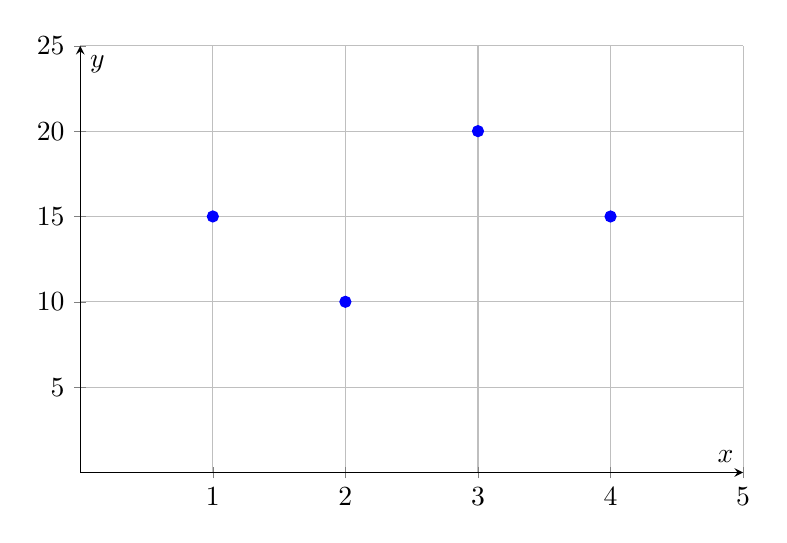
\begin{tikzpicture}
  \begin{axis}[
    axis lines = middle,
    xlabel = $x$,
    ylabel = $y$,
    xmin = 0, xmax = 5,
    ymin = 0, ymax = 25,
    grid = both,
    width=10cm,
    height=7cm,
    legend style={at={(0,1,..., 15)},anchor=north},
    xtick={0,1,...,16},
    ytick={0,5,...,25}
  ]
    % Puntos
    \addplot[only marks, mark=*, blue] coordinates {
      (1, 15) (2, 10) (3,20) (4,15)
    };
  \end{axis}
\end{tikzpicture}
\end{center}

La curva de regresión de X sobre Y son los puntos $(x_i, \bar  y_j)$, que son:
\[\{(3, 20), (2, 15), (2, 10)\}\]

\begin{center}
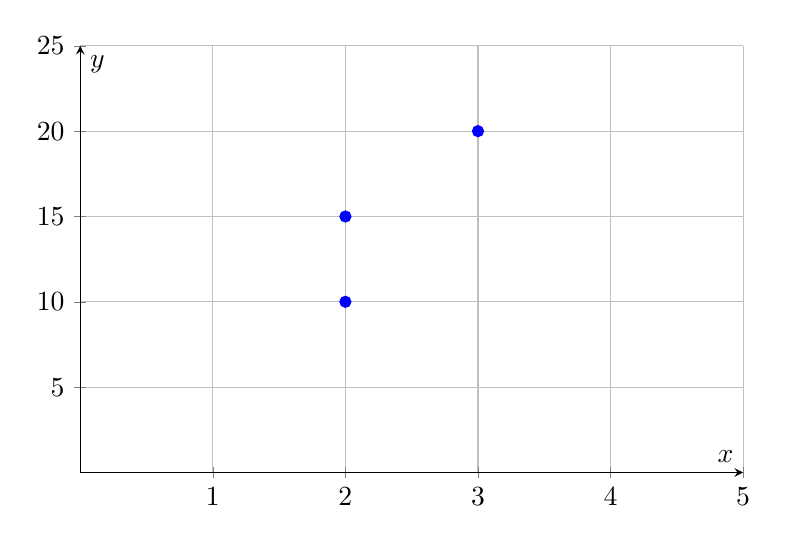
\begin{tikzpicture}
  \begin{axis}[
    axis lines = middle,
    xlabel = $x$,
    ylabel = $y$,
    xmin = 0, xmax = 5,
    ymin = 0, ymax = 25,
    grid = both,
    width=10cm,
    height=7cm,
    legend style={at={(0,1,..., 15)},anchor=north},
    xtick={0,1,...,16},
    ytick={0,5,...,25}
  ]
    % Puntos
    \addplot[only marks, mark=*, blue] coordinates {
      (3, 20) (2, 15) (2, 10)
    };
  \end{axis}
\end{tikzpicture}
\end{center}

\title{Distribución B}\\

La curva de regresión de Y sobre X son los puntos $(\bar x_i, y_j)$, que son:
\[\{(1, 15), (2, 10), (3, 20)\}\]

\begin{center}
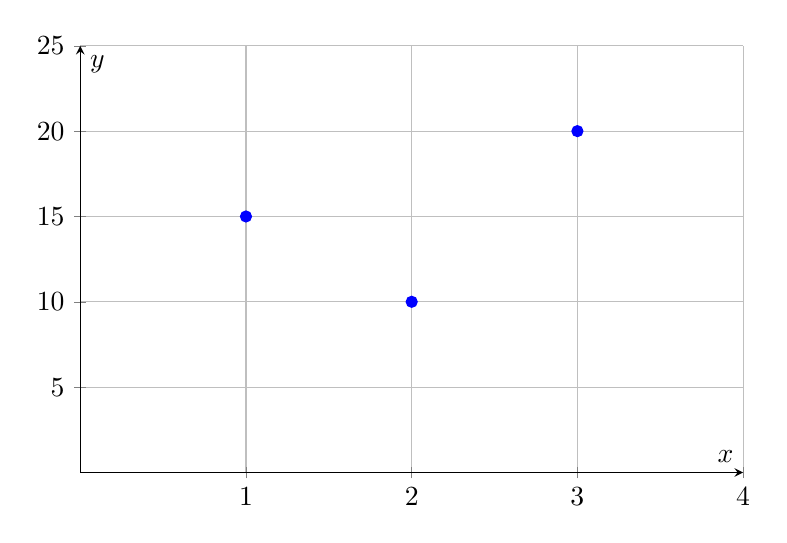
\begin{tikzpicture}
  \begin{axis}[
    axis lines = middle,
    xlabel = $x$,
    ylabel = $y$,
    xmin = 0, xmax = 4,
    ymin = 0, ymax = 25,
    grid = both,
    width=10cm,
    height=7cm,
    legend style={at={(0,1,..., 15)},anchor=north},
    xtick={0,1,...,16},
    ytick={0,5,...,25}
  ]
    % Puntos
    \addplot[only marks, mark=*, blue] coordinates {
      (1, 15) (2, 10) (3,20)
    };
  \end{axis}
\end{tikzpicture}
\end{center}

La curva de regresión de X sobre Y son los puntos $(x_i, \bar  y_j)$, que son:
\[\{(3, 20), (1, 15), (2, 10)\}\]

\begin{center}
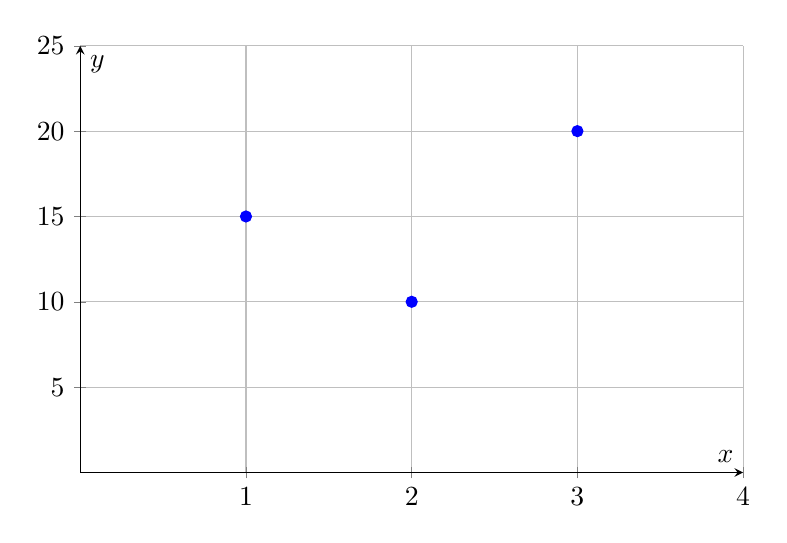
\begin{tikzpicture}
  \begin{axis}[
    axis lines = middle,
    xlabel = $x$,
    ylabel = $y$,
    xmin = 0, xmax = 4,
    ymin = 0, ymax = 25,
    grid = both,
    width=10cm,
    height=7cm,
    legend style={at={(0,1,..., 15)},anchor=north},
    xtick={0,1,...,16},
    ytick={0,5,...,25}
  ]
    % Puntos
    \addplot[only marks, mark=*, blue] coordinates {
      (3, 20) (1, 15) (2, 10)
    };
  \end{axis}
\end{tikzpicture}
\end{center}

\title{Distribución C}\\

La curva de regresión de Y sobre X son los puntos $(\bar x_i, y_j)$, que son:
\[\{(1, 17,5), (2, 10), (3, 20)\}\]

\begin{center}
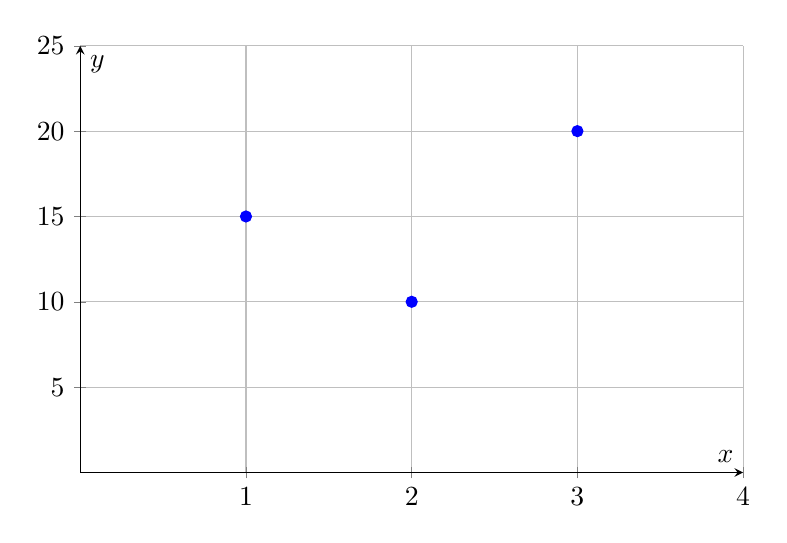
\begin{tikzpicture}
  \begin{axis}[
    axis lines = middle,
    xlabel = $x$,
    ylabel = $y$,
    xmin = 0, xmax = 4,
    ymin = 0, ymax = 25,
    grid = both,
    width=10cm,
    height=7cm,
    legend style={at={(0,1,..., 15)},anchor=north},
    xtick={0,1,...,16},
    ytick={0,5,...,25}
  ]
    % Puntos
    \addplot[only marks, mark=*, blue] coordinates {
      (1, 15) (2, 10) (3,20)
    };
  \end{axis}
\end{tikzpicture}
\end{center}

La curva de regresión de X sobre Y son los puntos $(x_i, \bar  y_j)$, que son:
\[\{(1,25), (1, 15), (2, 20), (3, 10)\}\]

\begin{center}
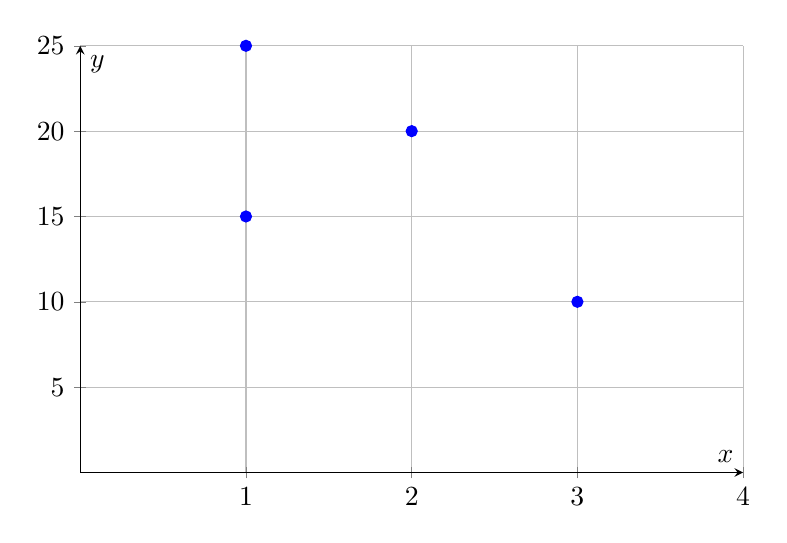
\begin{tikzpicture}
  \begin{axis}[
    axis lines = middle,
    xlabel = $x$,
    ylabel = $y$,
    xmin = 0, xmax = 4,
    ymin = 0, ymax = 25,
    grid = both,
    width=10cm,
    height=7cm,
    legend style={at={(0,1,..., 15)},anchor=north},
    xtick={0,1,...,16},
    ytick={0,5,...,25}
  ]
    % Puntos
    \addplot[only marks, mark=*, blue] coordinates {
      (1,25) (1, 15) (2, 20) (3, 10)
    };
  \end{axis}
\end{tikzpicture}
\end{center}

\section*{Ejercicio 8}
\begin{center}
\begin{tabular}{c|cccc}
X $\backslash$ Y & 1 & 2 & 3 & 4 \\
\hline
1 & 1 & 2 & 0 & 0 \\
2 & 1 & 2 & 3 & 1 \\
3 & 0 & 1 & 2 & 6 \\
4 & 0 & 0 & 2 & 3 \\
\end{tabular}
\end{center}

\begin{enumerate}
    \item[a)] Determinar las rectas de regresión.
    \item[b)] \textquestiondown Es apropiado suponer que existe una relación lineal entre las variables?
    \item[c)] Predecir, a partir de los resultados, el número de balanzas que puede esperarse en un puesto con seis dependientes. \textquestiondown Es fiable esta predicción?
\end{enumerate}

\begin{enumerate}
    \item[a)] Determinar las rectas de regresión.\textquestiondown Es fiable esta predicción?
\end{enumerate}

\begin{center}
\resizebox{.9\textwidth}{!}{
\begin{tabular}{c|cccc|c||c|c|c|c}
X $\backslash$ Y & 1 & 2 & 3 & 4 & $n_{i.}$ & $x_in_{i.}$ & $n_{i.}(x_i-\bar x)^2$  & $\sum n_{ij} y_{j.}$ & $x_i\sum n_{ij} y_{j.}$ \\
\hline
1 & 1 & 2 & 0 & 0 & 3 & 3 & 8,333 & 5 & 5\\
2 & 1 & 2 & 3 & 1 & 7 & 14 & 3,1111 & 14 & 28\\
3 & 0 & 1 & 2 & 6 & 9 & 27 & 1 & 32 & 96\\
4 & 0 & 0 & 2 & 3 & 5 & 20 & 8,8888 & 18 & 72\\
\hline
$n_{.j}$ & 2 & 5 & 7 & 10 & 24 & 64 & 21,333 &  & 201\\
\hline
$n_{.j}y_j$ & 2 & 10 & 21 & 40 & 73 & & & &\\
\hline
$n_{.j}(y_l-\bar y)^2$ & 8,336 & 5,4246 & 0,0121 & 9, 1853 & 23,06693 & & &\\
\end{tabular}
}
\end{center}

Con los datos de la tabla calculamos las medias: $\bar x = 2,666$, $\bar y = 3,0416$\\
Entonces, las varianzas son: $\sigma_x^2 = 0,8888$, $\sigma_y^2 = 0,961122$\\
Ahora calculamos la covarianza: $\sigma_{xy}=m_{11} - \bar x \bar y = 8,70833 - 8,1109 = 0,60369$\\
Con todo esto, podemos calcular las rectas de regresión:\\
\[y = \frac{\sigma_{xy}}{\sigma_x^2}x+(\bar y -\frac{\sigma_{xy}}{\sigma_x^2})\bar x = 0,6791x+1,23055\]
\[x = \frac{\sigma_{xy}}{\sigma_y^2}y+(\bar x -\frac{\sigma_{xy}}{\sigma_y^2})\bar y = 0,6281+0,7562\]

\begin{enumerate}
    \item[b)] \textquestiondown Es apropiado suponer que existe una relación lineal entre las variables?
\end{enumerate}

Para ver si es apropiado suponer que existe una relación lineal entre las variables, tenemos que calcular el coeficiente de correlación lineal $r^=\frac{\sigma_{xy}}{\sigma_x\sigma_y} = 0,648$, que no se acerca mucho a 1, por lo que no es adecuado suponer que existe una correlación lineal.\\

\begin{enumerate}
    \item[c)] Predecir, a partir de los resultados, el número de balanzas que puede esperarse en un puesto con seis dependientes. \textquestiondown Es fiable esta predicción?
\end{enumerate}

La recta de regresión sólamente tiene poder de predicción dentro del conjunto donde se encuentran los datos, por lo que sería absurdo intentar usar la recta de regresión calculada entre 1 y 4 dependientes para predecir lo que ocurriría con 6 dependientes, ya que estaríamos intentando suponer fuera la capacidad de predecir de la recta, donde no tendríamos seguro que esta sea la recta que minimice el error cuadrático en $Y=6$ (además, si se recogen los datos para 6 dependientes, muy probablemente la recta sea distinta).\\

Si suponemos que  la tendencia continúa, entonces $x= 0,6281 * 6 + 0,7562 = 4,5248$ balanzas.\\

Aun así, incluso en el caso de que tuviésemos los datos disponibles y de algún modo la tendencia continuase como en la suposición, el coeficiente de correlación lineal es demasiado bajo como para suponer que las variables están correlacionadas linealmente, lo que significa que la recta no es capaz de predecir el número de balanzas que pueden esperarse ni aún dentro del intervalo [1, 4], menos aún fuera de él.\\


\section*{Ejercicio 9}
\begin{center}
\begin{tabular}{c|ccccc}
X $\backslash$ Y & (10,20] & (20,25] & (25,30] & (30,35] & (35,40] \\
\hline
(15,18] & 3 & 2 & 3 & 0 & 0 \\
(18,21] & 0 & 4 & 2 & 2 & 0 \\
(21,24] & 0 & 7 & 10 & 6 & 1 \\
(24,27] & 0 & 0 & 2 & 5 & 3 \\
\end{tabular}
\end{center}

Estudiar la interdependencia lineal entre ambas variables.\\

Para ver la interdependencia (o correlación) lineal entre ambas variables, tenemos que calcular el coeficiente de correlación lineal $r=\frac{\sigma_{xy}}{\sigma_x\sigma_y}$. Para ello, calculamos la tabla de las distribuciones marginales para calcular ambas varianzas y la covarianza de la distribución:\\

\begin{center}
\resizebox{.95\textwidth}{!}{
\begin{tabular}{c|ccccc|c||c|c|c|c|c}
X $\backslash$ Y & (10,20] & (20,25] & (25,30] & (30,35] & (35,40] & $n_{i.}$ & $x_i$ & $n_{i.}x_i$ & $n_{i.}(x_i-\bar x)^2$ & $\sum n_{ij}y_j$ & $x_i\sum n_{ij}y_j$\\
\hline
(15,18] & 3 & 2 & 3 & 0 & 0 & 8 & 16,5 & 132 & 213,0048 & 172,5 & 2846,25\\
(18,21] & 0 & 4 & 2 & 2 & 0 & 8 & 19,5 & 156 & 37,3248 & 210 & 4095\\
(21,24] & 0 & 7 & 10 & 6 & 1 & 24 & 22,5 & 540 & 16,9344 & 665 & 14962,5\\
(24,27] & 0 & 0 & 2 & 5 & 3 & 10 & 25,5 & 255 & 147,456 & 330 & 8415\\
\hline
$n_{.j}$ & 3 & 13 & 17 & 13 & 4 & 50 & & 1083 & 414,72 & & 30318,75\\
\hline
$y_j$ & 15 & 22,5 & 27,5 & 32,5 & 37,5 & & & & &\\
\hline
$n_{.j}y_j$ & 45 & 292,5 & 467,5 & 422,5 & 150 & 1377,5 & & & &\\
\hline
$n_{.j}(yj-\bar x)^2$ & 472,5075 & 331,5325 & 0,0425 & 318,5325 & 396,01 & 1518,625 & & & &\\
\end{tabular}
}
\end{center}

Con los datos de la tabla, calculamos $\bar x =21,66$, $\bar y = 27,55$, $\sigma_x^2= 8,2944$ $\sigma_y^2 = 30,3725$, $m_{11} = 606,375$\\
Ahora, con los datos anteriores, calculamos la covarianza $\sigma_{xy}= 9,642$.\\
Finalmente, calculamos el coeficiente de correlación lineal $r=\frac{\sigma_{xy}}{\sigma_x\sigma_y} = \frac {9,642}{2,88*5,51125} = 0,654849$.\\
Como $r$ no se acerca a -1 ni a 1, no sería adecuado suponer una interdependencia lineal entre las dos variables.

\section*{Ejercicio 10}
Calcular el coeficiente de correlación lineal de dos variables cuyas rectas de regresión son:

\begin{itemize}
    \item $x + 4y = 1$
    \item $x + 5y = 2$
\end{itemize}

Sabemos que el producto de las dos pendientes da como resultado el coeficiente de determinación lineal $r^2$.\\
Como nos han dado las rectas de regresión pero no sabemos cuál corresponde a cada variable, tenemos en cuenta que el el coeficiente de determinación $0\leq r^2 \leq 1$, por lo que la única opción que tendría sentido es que las rectas sean:

\begin{itemize}
    $x=-4y+1$\\
    
    \\$y=\frac{-x+2}{5}$\\
\end{itemize}

Por lo que ahora podemos obtener que $r^2=a*a' = -4 * \frac{-1}{5}=0,8$.
Finalmente, para averiguar el coeficiente de correlación lineal de las dos variables, tenemos que $r=\sqrt{r^2}$ con el signo de la covarianza. En este caso, ese signo lo podemos ver claramente en la pendiente de ambas rectas de regresión (que además siempre será el mismo):\\
Si tomamos por ejemplo la recta  $x=-4y+1$, la pendiente $-4=\frac{\sigma_{xy}}{\sigma^2_{y}}$, y como $\sigma^2_{y}$ siempre es positivo, entonces la covarianza $\sigma_{xy}$ será negativa, por lo que $r=-\sqrt{r^2}=0,89442$

\section*{Ejercicio 11}
Consideremos una distribución bidimensional en la que la recta de regresión de $Y$ sobre $X$ es $y = 5x - 20$, y
\[ \sum y_j^2 n_{.j} = 3240. \]

Distribución marginal de $X$:
\begin{center}
\begin{tabular}{c|cccc}
$x_i$ & 3 & 5 & 8 & 9 \\
$n_{i.}$ & 5 & 1 & 2 & 1 \\
\end{tabular}
\end{center}

Determinar la recta de regresión de $X$ sobre $Y$, y la bondad de los ajustes lineales.

\begin{center}
\begin{tabular}{c|cccc|c}
$x_i$ & 3 & 5 & 8 & 9 &\\
\hline
$n_{i.}$ & 5 & 1 & 2 & 1 &-\\
$x_in_i$ & 15 & 5 & 16 & 9 & 45\\
$n_i(x_i-\bar x)^2$ &20&0&18&16&54\\
\end{tabular}
\end{center}

Simplemente con la distribución marginal de la variable x, ya podemos obtener la media $\bar x=\frac{1}{9} \sum\limits_{i=1}^4 x_in_i = \frac{45}{9}=5$, y la varianza de x $\sigma^2_x=\frac{1}{9} \sum\limits_{i=1}^4 n_i(x_i- \bar x)^2 = \frac{54}{9}=6$\\
Ahora, como ya tenemos la varianza de x, podemos calcular la covarianza utilizando la recta de regresión de Y sobre X dado que su pendiente, $5=\frac{\sigma_{xy}}{\sigma_x^2}$, por lo que $\sigma_{xy}=5*6=30$. Además, como el punto $(\bar x, \bar y)$ siempre pertenece a la recta, podemos obtener también de la recta que $\bar y=5(5) - 20 = 5$.\\
Finalmente, lo último que necesitamos lo podemos obtener de $ \sum y_j^2 n_{.j} = 3240. \ =n* m_{02}$, ya que $\sigma_y^2= m_{02} -m_{01}^2=\frac{3240}{9}-5^2 = 335$.\\
Ahora que tenemos todo lo necesario, calculamos la recta de regresión de X sobre Y: $x= \frac{\sigma_{xy}^2}{\sigma_y^2}y + (\bar x -\frac{\sigma_{xy}^2}{\sigma_y^2} \bar y)= 0,0896y+ 4,5522$\\

Para calcular la bondad de los ajustes lineales, debemos calcular el coeficiente de determinación lineal $r^2=(\frac{\sigma_{xy}}{\sigma_x \sigma_y})^2 = 0,4478$, lo que significa que el 44,78\% de la variablidad está explicada por las rectas, mientras que el resto son residuos.

\section*{Ejercicio 12}
Datos estadísticos sobre 24 trayectos de un avión DC-9:
\[ \sum y_i = 219.719, \quad \sum y_i^2 = 2396.504, \quad \sum x_i y_i = 349.486, \]
\[ \sum x_i = 31.470, \quad \sum x_i^2 = 51.075, \quad \sum x_i^2 y_i = 633.993, \]
\[ \sum x_i^4 = 182.977, \quad \sum x_i^3 = 93.6 \]

$Y$: consumo total de combustible (miles de libras), $X$: duración del vuelo (horas).

\begin{enumerate}
    \item[a)] Ajustar modelo $Y = aX + b$. Estimar el consumo total para un programa de 100 vuelos de media hora, 200 de una hora y 100 de dos horas. \textquestiondown Es fiable?

    El ajuste lineal tiene la fórmula 
    $$y=\bar y + \frac {\sigma_{xy}}{\sigma_x^2}(x-\bar x)$$
    Encontramos las expresiones para los datos que necesitamos:
    $$\bar x=\frac {\sum x_i}{n} = 1.31125$$
    $$\bar y=\frac {\sum y_i}{n} = 9.1549$$
    $$\sigma_x^2=\frac {\sum x_i^2}{n}-\bar x^2 = 0.40875$$
    $$\sigma_y^2=\frac {\sum y_i^2}{n}-\bar y^2 = 16.04104$$
    $$\sigma_{xy}=\frac {\sum x_iy_i}{n}-\bar x\bar y = 2.55747$$

     $$y=\bar y + \frac {\sigma_{xy}}{\sigma_x^2}(x-\bar x) \Rightarrow y=9.1549 + \frac {2.55747}{0.40875}(x-1.31125) = 0.95064 + 6.2568x$$

    Estimamos el consumo para 100 vuelos de media hora, 200 de una hora y 100 de dos horas:
    $$x=0.5 \Rightarrow y= 100*(0.95064 + 6.2568*0.5)=407.904$$
    $$x=1 \Rightarrow y= 200*(0.95064 + 6.2568*1)=1441.488$$
    $$x=2 \Rightarrow y= 100*(0.95064 + 6.2568*2)=1346.424$$
    El consumo será la suma de los 3 (En miles de libras):
    $$407.904+1441.488+1346.424= 3195.816$$

    Y calculamos $r^2$ para comprobar la fiabilidad de la recta de regresión:
    $$r^2=\frac{\sigma_{xy}^2}{\sigma_x^2\sigma_y^2}= \frac{2.55747^2}{0.40875*16.04104}= 0,997545$$
    Como $r^2$ es muy cercano a $1$, podemos afirmar que el ajuste lineal calculado es muy fiable.


    \item[b)] Ajustar modelo $Y = a + bX + cX^2$. Repetir la estimación del apartado anterior.

    Para obtener la Parábola de regresión de y sobre x, necesitamos resolver el siguente sistema de ecuaciones:
    
    \begin{equation}
    \left\{
    \begin{array}{l}
    m_{01} = a + bm_{10} + cm_{20} \\
    m_{11} = am_{10} + bm_{20} +cm_{30}\\
    m_{21} =  am_{20} +bm_{30} + cm_{40}\\
    \end{array}
    \right.
    \end{equation}
    
    $$m_{01} = \bar y = 9.1549$$
    $$m_{11} = \frac {\sum x_iy_i}{n}= 14.5619$$
    $$m_{21} = \frac {\sum x_i^2y_i}{n} =26.41637$$
    $$m_{10} = \bar x= 1.31125$$
    $$m_{20} = \frac {\sum x_i^2}{n}=2.1281$$
    $$m_{30} = \frac {\sum x_i^3}{n}=3.9$$
    $$m_{40} = \frac {\sum x_i^4}{n}= 7.62404$$

    Y el sistema queda como:
    \begin{equation}
    \left\{
    \begin{array}{l}
    9.1549 = a + 1.31125b + 2.1281c \\
    14.5619 = 1.31125a + 2.1281b + 3.9c\\
    26.41637 =  2.1281a +3.9b + 7.62404c\\
    \end{array}
    \right.
    \end{equation}

    Resolviendo la ecuación, obtenemos los coeficientes de la parábola. El ajuste nos queda como:
    $$y= -0,10596x^2 + 6,54482x +0,79855$$

    Estimamos el consumo para 100 vuelos de media hora, 200 de una hora y 100 de dos horas:
    $$x=0.5 \Rightarrow y= 100*(-0,10596*0,5^2 + 6,54482*0.5 +0,79855)= 404.447$$
    $$x=1 \Rightarrow y= 200*(-0,10596 + 6,54482 +0,79855)=1447.482$$
    $$x=2 \Rightarrow y= 100*(-0,10596*4 + 6,54482*2 +0,79855)=1346.435$$
    El consumo será la suma de los 3 (En miles de libras):
    $$404.447+1447.482+1346.435= 3198.364$$
    
    \item[c)] \textquestiondown Cuál de los dos modelos se ajusta mejor? Razonar la respuesta.

    Los dos ajustan la regresión de manera muy similar, sin embargo, como la parábola de regresión tiene coeficiente de grado 2 no nulo, quiere decir que la mejor aproximación a la distribución no será la de grado 1, por lo que la parábola es marginalmente mejor que la recta.
    
\end{enumerate}

\section*{Ejercicio 13}
Ajustar una hipérbola equilátera a los siguientes datos (curva de Engel):
\begin{center}
\begin{tabular}{c|cccc}
X (miles €) & 10 & 12.5 & 20 & 25 \\
Y (euros) & 50 & 90 & 160 & 180 \\
\end{tabular}
\end{center}

Cuantificar la bondad del ajuste.\\

Tenemos una población con n=4 , con $n_{ij}=1 \forall i,j =1,2,3,4$. El ajuste en forma de hipérbola tiene la forma $y=\frac{a}{x} + b$. Por tanto, transformamos a partir del ajuste lineal la variable $x$ a $Z=\frac{1}{x}$:
\begin{center}
\begin{tabular}{c|cccc}
X (miles €) & 10 & 12.5 & 20 & 25 \\
Y (euros) & 50 & 90 & 160 & 180 \\
\hline
$Z=\frac{1}{x}$ & 0.1 & 0.08 & 0.05 & 0.04\\
\end{tabular}
\end{center}

Realizamos el ajuste lineal con los nuevos datos:
$$\bar z= \frac {\sum n_iz_i}{n}=0.0675$$
$$\bar y=\frac {\sum n_iy_i}{n}= 120$$
$$\sigma_z^2=\frac {\sum n_iz_i^2}{n}-\bar z^2 = 0.00056875$$
$$\sigma_y^2=\frac {\sum n_iy_i^2}{n}-\bar y^2 = 2750$$
$$\sigma_{zy}=\frac {\sum n_{ij}z_iy_i}{n}-\bar y \bar z = -1.25$$

$$y= a+bz = \bar y + \frac {\sigma_{zy}}{\sigma_z^2}(z-\bar z) \Rightarrow y=120 + \frac {-1.25}{0.00056875}(z-0.0675) = 268.351 -2197.802z$$

Y deshaciendo el cambio de variable, tenemos que:
$$y= a+bz = a +\frac{b}{x} = 268.351 -\frac{2197.802}{x}$$

Para comprobar la bondad del ajuste, calculamos 
$$r^2 = \frac{\sigma_{zy}^2}{\sigma_z^2\sigma_y^2}=\frac{-1.25^2}{0.00056875*2750}=0.999$$

Que, como es muy próximo a 1, nos dice que la hipérbola de regresión es muy fiable para ajustar los datos de la distribución.

\section*{Ejercicio 14}
Datos sobre renta disponible mensual ($X$, cientos de euros) y gasto en espectáculos ($Y$, euros):
\begin{center}
\begin{tabular}{c|cccccc}
Y & 30 & 50 & 70 & 80 & 120 & 140 \\
X & 9 & 10 & 12 & 15 & 22 & 32 \\
\end{tabular}
\end{center}

Explicar el comportamiento de $Y$ por $X$ mediante:


\begin{enumerate}
    \item[a)] Relación lineal.

    Calculamos los datos necesarios:
    $$\bar x= \frac {\sum n_ix_j}{n}=16.666$$
    $$\bar y=\frac {\sum n_iy_j}{n}= 81.666$$
    $$\sigma_x^2=\frac {\sum n_ix_i^2}{n}-\bar x^2 =  65.222$$
    $$\sigma_y^2=\frac {\sum n_iy_j^2}{n}-\bar y^2 = 1447.222$$
    $$\sigma_{xy}=\frac {\sum n_{ij}x_iy_j}{n}-\bar y \bar x =  293.888$$

    El ajuste será:
    $$y= \bar y + \frac {\sigma_{xy}}{\sigma_x^2}(x-\bar x) \Rightarrow y=81.666 + \frac {293.888}{65.222}(x-16.666) = 6.56729+ 4.5059x $$
    
    Para comprobar la bondad del ajuste, calculamos la varianza residual del ajuste. como estamos utilizando un ajuste lineal, se puede calcular utilizando $r^2$: 
    $$r^2 = \frac{\sigma_{xy}^2}{\sigma_x^2\sigma_y^2}=\frac{293.888^2}{65.222*1447.222}=0.9150$$
    $$\sigma_{ry}^2=(1-r^2)\sigma_y^2=122.98$$
    
    \item[b)] Hipérbola equilátera.

    Completamos la tabla con los cambios de variable necesarios para el apartado:
    
    \begin{center}
    \begin{tabular}{c|cccccc}
    Y & 30 & 50 & 70 & 80 & 120 & 140 \\
    X & 9 & 10 & 12 & 15 & 22 & 32 \\
    \hline
    $B=\frac{1}{x}$ & 0.111 & 0.1 & 0.08333 & 0.0667 & 0.0454545 & 0.03125 \\
    \end{tabular}
    \end{center}
    
    Calculamos los datos necesarios:
    $$\bar b= \frac {\sum n_ib_i}{n}=0.0729$$
    $$\sigma_b^2=\frac {\sum n_ib_i^2}{n}-\bar b^2 =  0.0008052$$
    $$\sigma_{by}=\frac {\sum n_{ij}b_iy_j}{n}-\bar y \bar b =  -1.0708$$

    El ajuste será:
    $$y= \bar y + \frac {\sigma_{xy}}{\sigma_x^2}(x-\bar x) \Rightarrow y=81.666 + \frac { -1.0708}{0.0008052}(b-0.0729) = 179.55 -1340.843b$$
    Y deshaciendo el cambio de variable, tenemos:
    $$y=179.55 -\frac{1340.843}{x}$$
    
    Para comprobar la bondad del ajuste, calculamos la varianza residual:
    $$r^2 = \frac{\sigma_{by}^2}{\sigma_b^2\sigma_y^2}=\frac{-1.0708^2}{0.0008052*1447.222}=0.98405$$
    
    $$\sigma_{ry}^2=(1-r^2)\sigma_y^2=27.46$$
    
    \item[c)] Curva potencial.
    Completamos la tabla con los cambios de variable necesarios para el apartado. En este caso, como la curva será de la forma $y=bx^a$, tendremos que cambiar las variables para que quede como una recta de la forma $y'=b+ax \Rightarrow ln(y)=ln(bx^a) = ln(b)+aln(x) = b'+ax'$:
    
    \begin{center}
    \begin{tabular}{c|cccccc}
    Y & 30 & 50 & 70 & 80 & 120 & 140 \\
    $Y'=ln(y)$ & 3.401 & 3.912 & 4.248 & 4.382 & 4.787 & 4.941\\
    \hline
    X & 9 & 10 & 12 & 15 & 22 & 32 \\
    $X'=ln(x)$ & 2.197 & 2.302 & 2.484 & 2.708 & 3.091 & 3.4657\\
    
    \end{tabular}
    \end{center}
    
    Calculamos los datos necesarios:
    $$\bar x'= \frac {\sum n_ix'_i}{n}=2.70795$$
    $$\bar y'= \frac {\sum n_iy'_j}{n}=4.2785$$
    $$\sigma_{x'}^2=\frac {\sum n_ix_i'^2}{n}-\bar x'^2 = 0.1994$$
    $$\sigma_{y'}^2=\frac {\sum n_iy_j'^2}{n}-\bar y'^2 = 0.268908$$
    $$\sigma_{x'y'}=\frac {\sum n_{ij}x_i'y_j'}{n}-\bar x' \bar y' = 0.2167$$

    El ajuste será:
    $$y'= \bar y' + \frac {\sigma_{x'y'}}{\sigma_{x'}^2}(x'-\bar x') \Rightarrow y'=4.2785 + \frac {0.2167}{0.1994}(x'-2.70795) = 1.33563 + 1.08675x'$$
    
    Y deshaciendo el cambio de variable, tenemos:
    $$y=e^{1.33563}x^{1.08675}= 3.8024x^{1.08675}$$
    
    Para comprobar la bondad del ajuste, calculamos la varianza residual:

    $$\sigma_{x'y}=\frac {\sum n_{ij}(y_j-f(xi))^2}{n}= 182.537$$
    
    \item[d)] Curva exponencial.
    Completamos la tabla con los cambios de variable necesarios para el apartado. En este caso, como la curva será de la forma $y=ba^x$, tendremos que cambiar las variables para que quede como una recta de la forma $y'=b+ax \Rightarrow ln(y)=ln(ba^x) = ln(b)+xln(a) = b'+a'x$:
    
    \begin{center}
    \begin{tabular}{c|cccccc}
    Y & 30 & 50 & 70 & 80 & 120 & 140 \\
    $Y'=ln(y)$ & 3.401 & 3.912 & 4.248 & 4.382 & 4.787 & 4.941\\
    \hline
    X & 9 & 10 & 12 & 15 & 22 & 32 \\
    
    \end{tabular}
    \end{center}
    
    Calculamos los datos necesarios:
    $$\bar x= \frac {\sum n_ix_i}{n}=16.666$$
    $$\bar y'= \frac {\sum n_iy'_j}{n}=4.2785$$
    $$\sigma_{x}^2=\frac {\sum n_ix_i^2}{n}-\bar x^2 = 65.222$$
    $$\sigma_{y'}^2=\frac {\sum n_iy_j'^2}{n}-\bar y'^2 = 0.268908$$
    $$\sigma_{xy'}=\frac {\sum n_{ij}x_iy_j'}{n}-\bar x \bar y' = 3.6699$$

    El ajuste será:
    $$y'= \bar y' + \frac {\sigma_{xy'}}{\sigma_{x}^2}(x-\bar x) \Rightarrow y'=4.2785 + \frac {3.6699}{65.222}(x-16.666) = 3.341+ 0.05627x$$
    
    Y deshaciendo el cambio de variable, tenemos:
    $$y=e^{3.341}e^{0.05627x}= 28.247x^{0.05627x}$$
    
    Para comprobar la bondad del ajuste, calculamos la varianza residual:
    $$\sigma_{x'y}=\frac {\sum n_{ij}(y_j-f(xi))^2}{n}= 361.71666$$
    
\end{enumerate}
\textquestiondown Qué ajuste es más adecuado?\\
El ajuste más adecuado será el que deje, de media, menos residuos con respecto a los valores que toma la distribución, es decir, el ajuste cuya varianza residual sea menor. En este caso, la hipérbola tiene un valor menor de varianza residual, por tanto, será elajuste más adecuado.


\end{document}
